\chapter{Conclusion and Future work}\label{ch:07Conclusion}
\paragraph{Conceptual problem formulation} is introduced in chapter \ref{ch:01Concept}. Where related work and goals are main focus, the goals have been fulfilled to some extent and some aspects needs additional work. 

\paragraph{The \emph{data fusion problem}} has been formulated in \ref{ch:02DataFusionProblem}, the three questions of \emph{visibility, reachability, and obstacle probability} have been confronted with deterministic approach shortcomings (sec. \ref{sec:deterministicApproachShortcommings}), where problem of \emph{LiDAR density} (fig. \ref{fig:P01CountOfLiDARHits}), \emph{map and detected obstacles fusion} (fig. \ref{fig:P02OvershadowedMapobstacle}), \emph{Intruder behaviour} (fig. \ref{fig:P03AdversaryProbabilitySpread}), and \emph{safety of passing trajectories} (fig. \ref{fig:P04SafetyOfPassingTrajectories}) have been opened.

\paragraph{The state of art} have been discussed in chapter \ref{03StateOfArt}. This chapter is taken from most parts \cite{alojzgomola2017}. It introduces the notion of UAV model in continuous time (\ref{eq:nonlinearsystem}) and in discrete time (\ref{eq:Discretegenericuavmodel}) The key concepts of reach sets are given in section \ref{s:ReachSets}. The reach set used further in $\mathscr{R}(\hat{x},t_i,t_{i_1})$ (\ref{eq:basicReachSetDefinition}), is point based reach set with restricted control. Movement automaton $\mathscr{MA}$ concept is introduced in section \ref{sec:movement automaton}, by definition \ref{def:movementAutomaton}. \emph{Movement automaton prediction stability} is given by definition \ref{def:maPredictionStability}. \emph{Movement automaton Lyapunov stability} is proven in section \ref{s:maLyapunov}. The other important properties, like \emph{controllability, robustness, observability} have been proven in \cite{frazzoli2000trajectory}.

\paragraph{The control framework based on reach sets} have been introduced in \cite{alojzgomola2017}. The complex topology scheme and communication is omitted in conclusion, only key modules for this work will be discussed. \emph{Obstacle avoidance} in terms of data fusion with dynamic obstacle sets $\mathscr{O}_D$, $O_M$, originating from various data sources $\mathscr{S}=\{s_1,s_2,\dots,s_k\}, k\in\N$. Movement constraints are mainly given by static uncharted obstacles and non-cooperative intruders. The main focus is on \emph{data fusion}. Usually multiple layer control concept is used. Control concept used for this work is in fig. \ref{fig:controlConceptIntro}.
\begin{figure}[H]
    \centering
    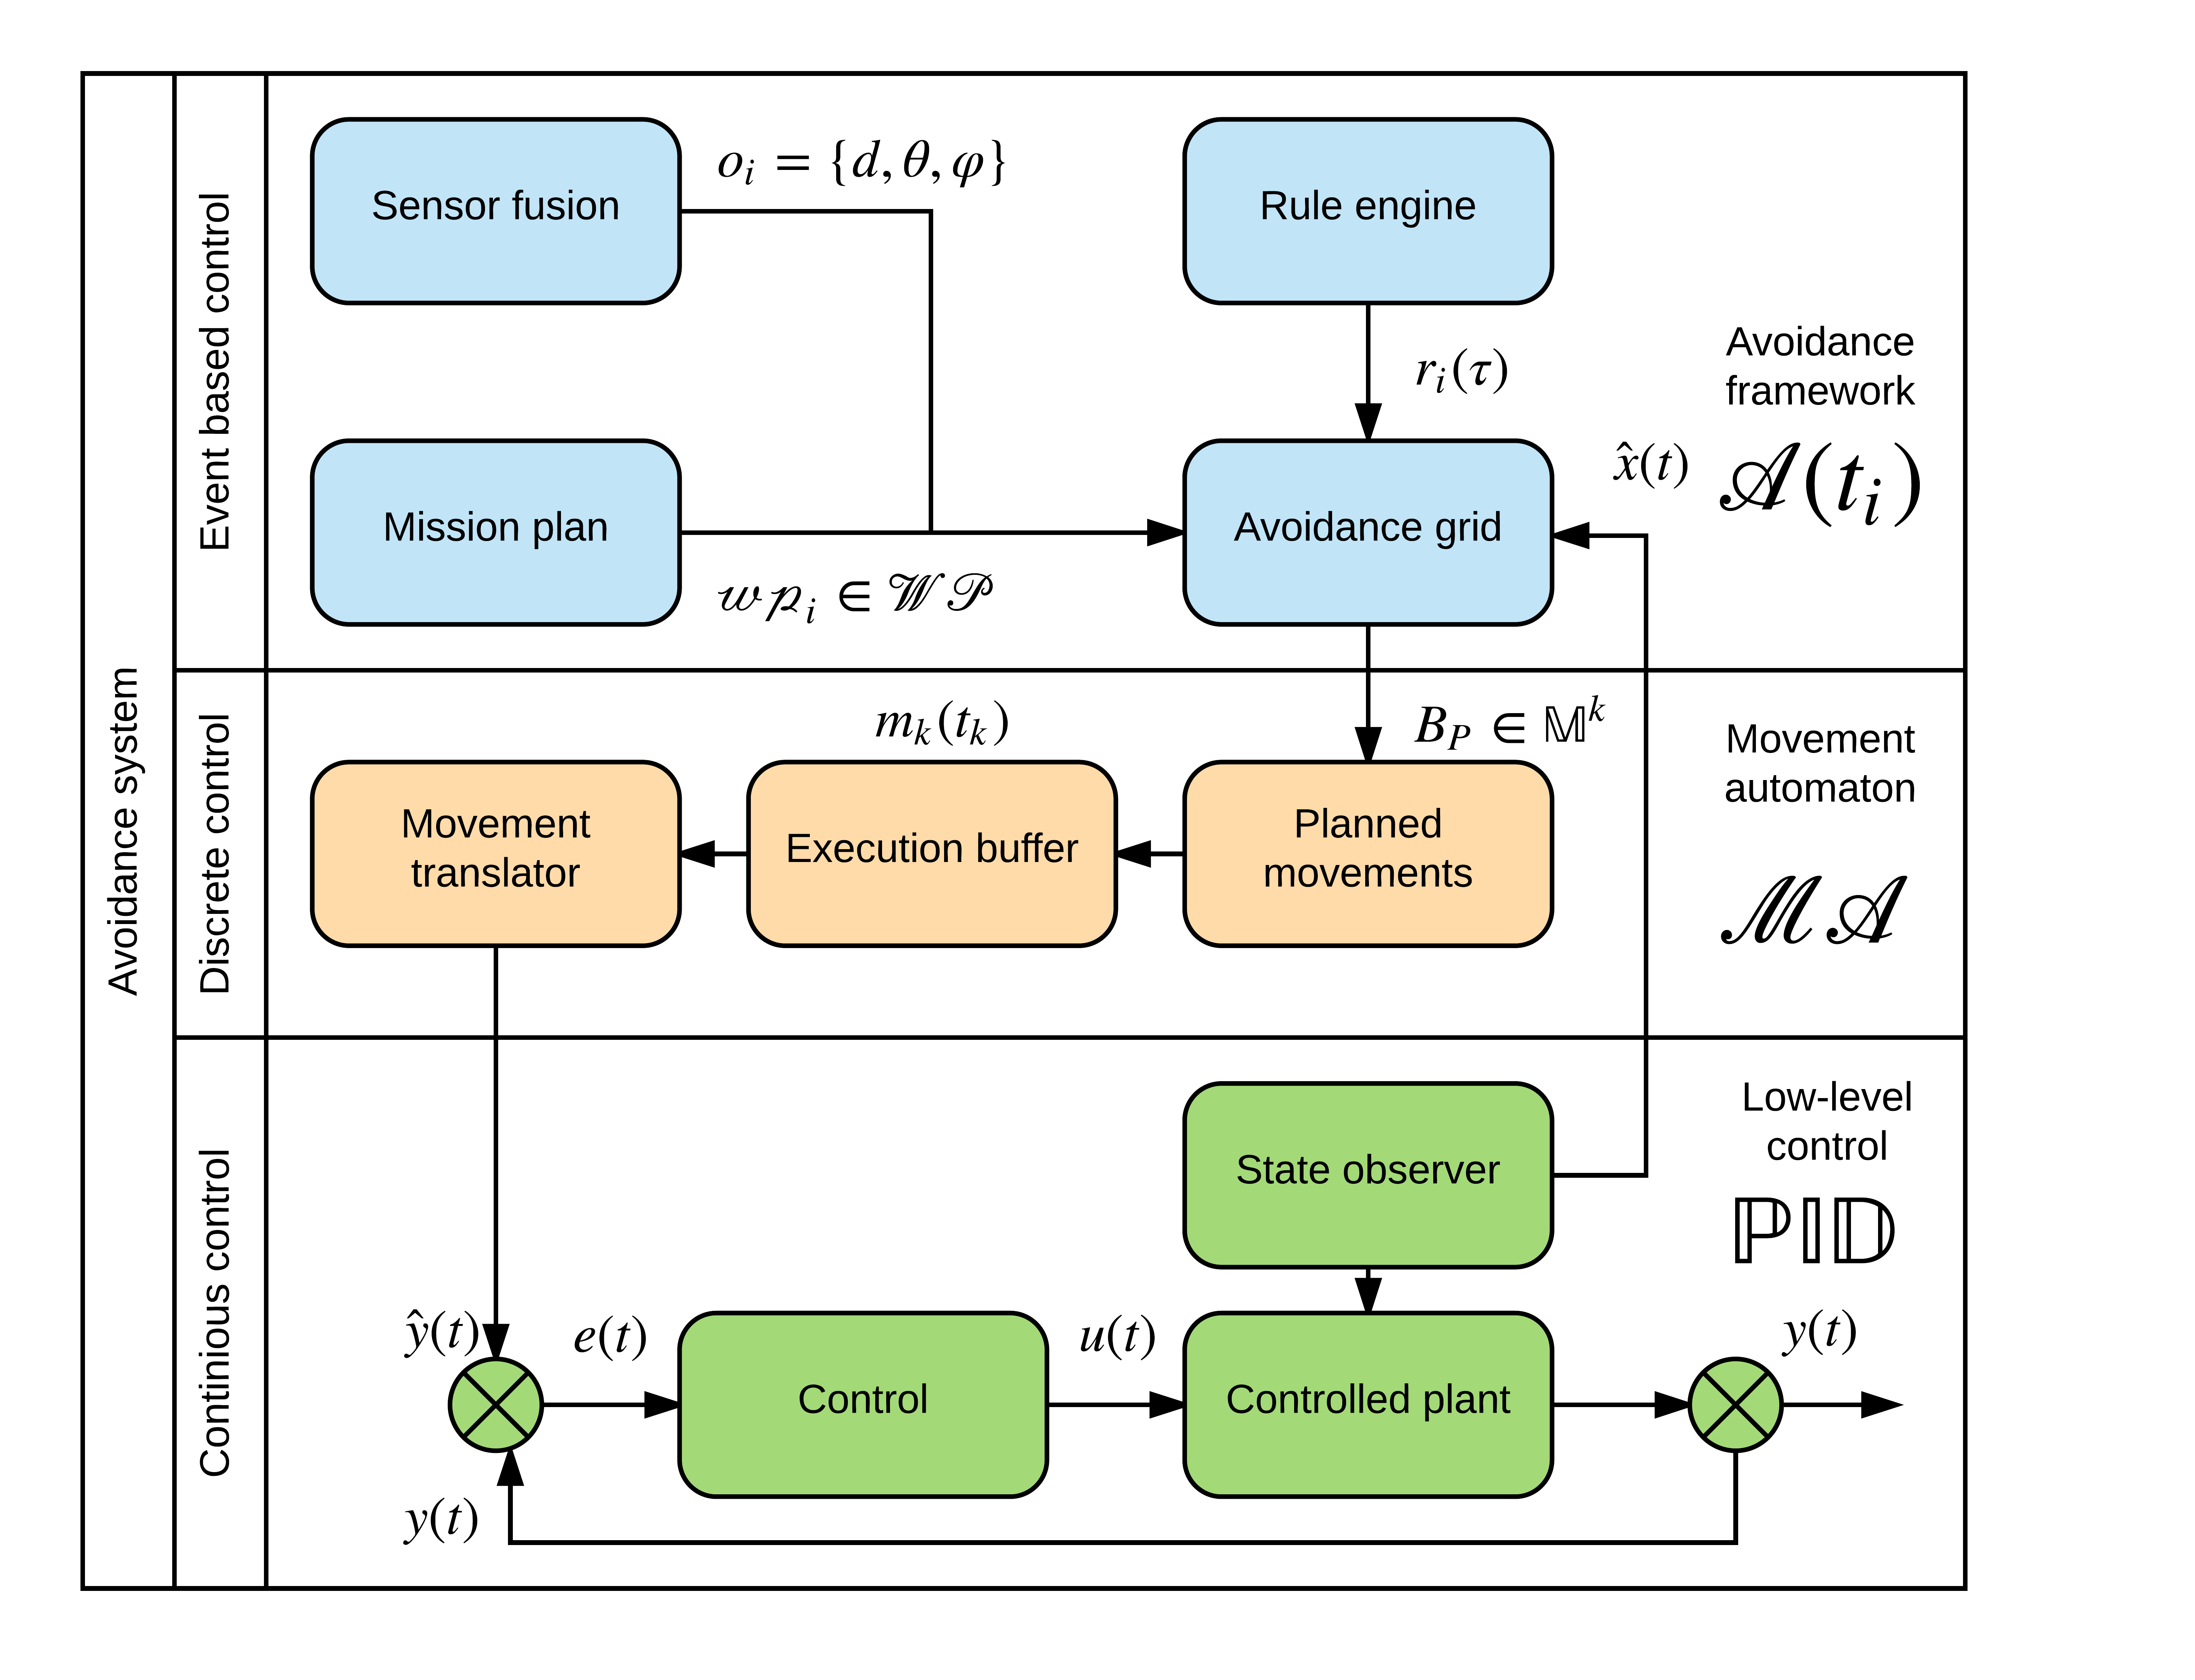
\includegraphics[width=.95\linewidth]{\FIGDIR/72_Control_Concept.png}
    \caption{Decision frame $\mathscr{D}(0)$.}
    \label{fig:controlConceptIntro}
\end{figure}

\noindent \emph{Event based control} module is responsible for high level decisions and mission execution. This module generates high level input commands which are optimal to given criterion. \emph{Event based control} consist from following artifacts:
\begin{enumerate}
    \item \emph{Sensor fusion} - fuses data from sensor system with observed system state $\hat{x}$, outputs detected obstacles $o_i\in\mathscr{O}$.
    \item \emph{Mission plan} - contains mission plan $\mathscr{WP}$, determines navigation goal waypoint $\mathscr{WP}_g$.
    \item \emph{Rule engine} - determines additional constraints for avoidance grid $\mathscr{A}(t_i)$, determines escape goal in avoidance grid $c_{i,j,k}$.
    \item \emph{Avoidance grid} - responsible for optimal path planning in partially known space, consumes observed system state $\hat{x}(t)$, rule engine decisions $r_i(\tau)$, obstacle set $o_i\in\mathscr{O}$ and goal waypoint $\mathscr{WP}_i$, produces avoidance command chain $B_p \in \mathbb{M}^k$.
\end{enumerate}

\emph{Discrete control} module is responsible for processing high level movement command chain $B_p \in \mathbb{M}^k$. It is implemented as special type of open hybrid automaton, movement automaton $\mathscr{MA}$. 

\emph{Continuous control} module is interfaces from \emph{avoidance} system via the movement automaton. The same is achieved with \emph{sensor fusion} module which is interfacing the sensor network $\mathscr{S}$ and avoidance grid $\mathscr{A}(t_i)$.

\paragraph{Problem of data fusion} is formulated in chapter \ref{ch:04ProblemFormulation}, outlining important \emph{general data fusion algorithm} proposal, section \ref{sec:general algorithm}. The identified probabilities and input artifacts are summarized in eq. \ref{eq:mainRatingInputs}. The \emph{main fusion algorithm} is proposed in eq. \ref{eq:mainRatingCalculation}. The new definition of \emph{reachability probability} $P_R$ bounded to trajectory $\mathscr{T}(x_0,B)\in\mathscr{R}$ have been established by definition \ref{def:ReachibilityProbabilityForTrajectory}, furthermore projected into cell $c_{i,j,k}\in\mathscr{A}$ reachability probability established by definition \ref{def:cellReachibilityProbability}.

\paragraph{Reduced reach set} calculation have been introduced due the calculation complexity of probabilistic distribution over full reach set. Concept of \emph{coverage ratio} $C_R$ (\ref{eq:reachSetCoverageRatio}) which considers \emph{trajectory footprint} (def. \ref{def:trajectoryFootprint}, \ref{def:trajectoryFootprintSet}). The \emph{constrained expansion procedure} (sec \ref{susbsec:ConstrainedExpansionProcedure}) have been developed to improve estimated reach set calculation. Three new procedures to reach set $\mathscr{R}(\hat{x},t_i,t_{i+1})$ have been developed:
\begin{enumerate}
    \item Chaotic reach set approximation (sec. \ref{s:chaoticApproximationReachSet}).
    \item Harmonic reach set approximation (sec. \ref{s:harmonicApproximationReachSet}).
    \item Combined reach set approximation (considered in testing) (sec .\ref{s:combinedReachSetApproximation}).
\end{enumerate}

\paragraph{Important results} are linked to research proposal goals:

\noindent\emph{Goal 1.: Universal interface for vehicle sensors} have been introduced in section \ref{sec:general algorithm}.

\noindent\emph{Goal 2.: Probabilistic model for avoidance grid} have been summarized in topics:
\begin{enumerate}
    \item\emph{Intruder intersection model} (sec. \ref{sec:intruderIntersectionModel}) introduces the concept of intruder intersection with avoidance grid. The notable are boundaries for cell entry (\ref{eq:cellEntryTime}) and cell leave time (\ref{eq:cellLeaveTime}) which enables to take time into account when calculating probability (\ref{eq:intruderIntersectionProbability}). Concept of base intersection probability have been defined for following intersection modes:
    \begin{enumerate}[a.]
        \item linear intersection model (\ref{eq:baseIntersectionProbabilityLineIntersectionType}),
        \item vehicle body volume intersection model (\ref{eq:baseIntersectionProbabilityBallIntersectionType}),
        \item conic spread intersection model (\ref{eq:spreadIntruderIntersectionProb}).
    \end{enumerate}
    \noindent Then \emph{general producible intersection model} (\ref{eq:intruderInCellProbabilityOneIntruder}) of one intruder $i\in\mathscr{I}$ has been defined combining the previously mentioned intersection modes of base probabilities and time constraints (\ref{eq:partialProbabilitiesIntruderSummary}). The intruder obstacle probability for single cell $c_{i,j,k}\in\mathscr{A}(t_i)$ and multiple intruders $i \in \mathscr{I}(\tau)$ has been given by (\ref{eq:intruderInCellProbability}).
    
    \item\emph{Detected obstacle probability} generic model for multiple sensors $s_k\in\mathscr{S}$ has been given by eq. \ref{eq:detectedObstacleProbability}. \textit{LiDAR hit formula} (\ref{eq:lidarHitFormula}) has been created for simple homogeneous rotary LiDAR sensor.
    
    \item\emph{Visibility probability} for sensor network $\mathscr{S}$ has been defined in eq. \ref{eq:FinalVisibilityProbability}.
    
    \item\emph{Map obstacle probability} is defined as combination of visibility and raw map obstacle probability (\ref{eq:finalMapObstacleProbability}).
\end{enumerate}

\emph{Goal 3.: Data fusion procedure} is proposed in section \ref{sec:general algorithm}.

\emph{Goal 4.: Comparison of probabilistic and deterministic approach} have been simulated in section \ref{sec:staticObstacleAvoidanceSimulation}. Detailed comparison with results from deterministic approach \cite{alojzgomola2017} are given in section \ref{sec:probabilisticModelEvaluation}. \emph{Avoidance performance} is compared in section \ref{sec:avoidancePerformacne}.

\paragraph{Future work} on probabilistic approach is mainly in partition of sensor fusion. Currently the sensor fusion for LiDAR and ADS-B have been proposed, but there is more ranging sensors which are not coherence with avoidance grid like LiDAR. 

\emph{Sensor fusion priority problem:} Vehicle can be equipped with various cooperative and non-cooperative sensors $s_1,s_2,\dots,s_4\in\mathscr{S}$. Which have some overlapped areas and some precision. It would be necessary to develop \emph{prioritized sensor fusion}, complex outline of this problem in deterministic context have been given by \cite{xiong2002multi}.

\paragraph{Reusable components for deterministic approach}: Probabilistic approach have introduced concepts of \emph{coverage ratio} $C_R$ and \emph{reduced reach set approximation}. These results can be used to reduce reach set complexity and improve scalability of deterministic approach \cite{alojzgomola2017}.

\emph{The intruder intersection model} can be reused in deterministic approach, where the step function to asset the reachability of cell. 
